\documentclass{article}
\usepackage{graphicx} % Required for inserting images
\usepackage{pdfpages}
\usepackage{url}
\title{4060 - T29: Real Time Networking \\ Student Log}

\author{Andrew Marinic - 7675509}
\date{January - April 2024}

\begin{document}

\maketitle
\newpage

\tableofcontents

\newpage

\section{Introduction}
\paragraph{Intro}
The following is a log or perhaps a journal of my efforts in COMP 4060 - T29 - Real Time Networking. I will break the document into sections for each Month and subsections for each week. Each day will contain a paragraph explaining what I had accomplished. 
\section{January}
\subsection{January 8-12}
\paragraph{Jan 8}
I did some preliminary reading of the documents provided on CAN networks. I only spent about an hour reading, little notes. 
\paragraph{Jan 11}
Dug into the data sheets. Started examining the UART drivers we need to build. Probably 30 mins or so taken aside. Industrial Project has hit the fan a bit and taken up more time. I set up a calendar for the group as we all have fairly tight schedules right now.
\subsection{January 15-19}
\paragraph{Jan 15}
We had an hour-long group meeting today. We discussed the pace of the project we would like to achieve. Send off an email to confirm some items and inform the Supervisor of our meeting availability. I started to dig into blinky again with the updated code. To my grief, I have switched to VScode and started to try and get the debugging working with the help of the other group members. I spent another hour or so getting the debugging to work in VScode, I stopped once I had the debugger open, openOCD via VScode. I started to get a little frustrated and had to finish my industrial project proposal so I stopped for the evening. I will discuss with the group for advice and continue later this week. 
\paragraph{Jan 17}
Today I spent around 4 hours deep-diving CAN and making notes on it. Then I proceeded to try and get debugging working one last time before asking for help. If I cannot accomplish this by, Friday I will reach out. I spent approx 1.5 hours on this, but more time was spent reading about it than coding. 

\paragraph{Jan 18}

Spent approximately 1 hour reading into the Curiosity Nano's CAN controller. I think I understand the requirements for setting up and how the INIT and CONFIG registers work together. 
\subsection{January 19-23}
\paragraph{JAN 22}
I spent about an hour and a half finishing my CAN notes which are visible in the Notes section. I have done some looking into coding the CAN controller of the curiosity nano. 
\begin{itemize}
    \item \url{https://github.com/MikroElektronika/mikrosdk_click_v2/tree/master/clicks/canfd3} Here is the CAN FD 3 example code. I gave it a quick browse for something valuable but was mainly looking for CAN controller init code keeping it in my back pocket  though
    \item \url{https://microchip-mplab-harmony.github.io/reference_apps/apps/sam_e51_cnano/same51n_mikroe_click/readme.html} I also gave themse projects a quick brows for the same as above, but I don't think any use the CAN controller just UART. 
    \item \url{https://microchip-mplab-harmony.github.io/reference_apps/apps/sam_e54_xpro/same54_can_usb_bridge/readme.html#hardware-used} I do however think there is something useful here. It uses the same micro controller so it should have INIT, read/write code, ect. This will take some digging though. 
    Today I put in approximately 3.5 hours into researching and documenting. 
\end{itemize}
\paragraph{JAN 24}
I tinkered more with debugging for about an hour or two this morning. It seems to be somewhat working but I am still not getting proper debugging and have no output from the debug calls. I will give it one last go. I think we will plan a group in person meeting, maybe input from the other students will help. I maybe just need to keep fresh eyes on it and stop getting frustrated and understand it better, but config files are frustrating to me. In a more productive note, I have started some framework for my drive code. I am going to clean up some of my I2C code for my gyro so I have a device to poll data from and send over the CAN network. This way I can make sure I understand the new systimer and clock speed a little better with something I understand. I suspect I will have to use some prescalers to compensate for the 60 times faster clock. I will do a commit at end of day and upload this as a pdf. 
\subsection{January 26 - February 1 }
\paragraph{JAN 29}
Today I continued my efforts of attempting to get the CAN0 controller initialized. I got some preliminary coding done with it. I sort of got confused with some of the usage documentation and searched for some reference code online. I am having serious troubles finding anyone who has used the CAN controller on a SAM E5 device and the same sam.h dependency. I continued by porting over more of my I2C code. In total I worked on this for about 2.5 hours today. GitHub will have a commit by end of day along with updated pdf. VS Code configs continue to delay progress, but not majorly. We have scheduled a virtual meeting for Wednesday January 31st.

\paragraph{JAN 31}
Today we had a group meeting. The minutes will be in the notes. Jacob helped me debug my debugger issues and it appears to be a bunch of version issues. I think its time to setup a Docker. I think Landon may have one. I spent about an hour in the meeting and and additional hour working on the silly version stuff. 
\section{February}
\subsection{February 5-9}
\paragraph{FEB 5} I spent some time attempting Landons docker but I quickly abandoned that when I had the realization that python source has a make command to do an altinstall alongside the main install. This finally got gdb working, but my debug still does not work. It no longer hangs as it did before but I an getting no response back from the device. Perhaps my USB cable actually is bad. I will attempt a few other to see if this fixes the problem. Only about an hour spent today with no major coding. Intellisense still broken and I hate VS code. 
\paragraph{FEB 7} I finally have all my old code ported over. I am now testing. I suspect the new sysTimer settings have complicated things. The button no longer works. I quickly re-installed the very cool named project kyber and tested the button with my old code. It works "flawlessly" in the sense of it works as it did before. Button works, gyro communicates. I have even tried directly copying and not reformatting my code, again does not work. Must investigate settings more but wont let it slow me down for now. Here is my game plan:
\begin{itemize}
    \item Finish CAN drivers
    \item Get I2C get gyro data on a schedule
    \item Attempt to send gyro data over CAN
\end{itemize}
As far as continuing to debug my old code, I am going to attempt to set up another timer and PWM it to see exactly how fast the timers are moving. The force is with me, debug is now working, I tried some more stuff and eventually put in a new usb cable, not sure if that was it. Maybe my uhhhhh usb cable was "bad" or "crap" or other less civil synonyms. I can now remove this burden from my todo list. I can now use this for debugging my button and other code. Had group meeting. Finished up some code before I called it for the day and changed focus. 
\subsection{Feb 25th - 28th}
\paragraph{FEB 25} Back into the swing of it. I have continued to follow the sample code I have followed. Today I fixed the circular reference in my I2C code. I made some circular references when I was separating my I2C code from my just gyro code. I re-merged them for now as I wanted to see if the I2C is still working with the systimer. I can't get messages like I used to in my project but I suspect its a buad rate issue. I did a small amount of tinkering to see if it was a quick fix. Unfortunately I didn't manage to send anything other than a start signal. I will tinker with this more another time. I shifted my focus to the CAN controller for an  3 hours. I followed along with the example code that Jacob had shown me a in our Jan 31st meeting. I also discussed some of the topics with Jacob on discord. I started to use the value assignment functions from sam.h as they are significantly better at bit bashing the registers all at once. I set the quanta with small values for testing. I have also turned on the feed back loop. The data analyzer isn't showing me anything interesting yet. I have tried to use the debugger to set my base ram location for messages, but have not managed to get the same address back. Jacob and I have agreed to a discord discussion on Wednesday, we wait for Landon's response. The debugger is proving very valuable. I will pick Jacobs brain more on this ram issue if I can't figure it out before then. Today in total I worked on the project for approximately 4.5 hours.
\paragraph{FEB 28} \textbf{We had a group meeting today:} All attended. Landon appears to be having the same power issues with their board. Jacob and I provided sanity check conversation such as "No that works for me" sort of thing. Landon is trying a new bread board, and I have offered for him to test on my board Tues/Thursdays when we are on campus at the same time. The three of us quickly discussed the logistics of initializing (and how simple it is) and the logic of sending messages. After this Landon had to leave (about 45 min to an hour). We discussed Jacob not being able to get CAN+/- to work together. Jacob and I discussed some debugging methodologies. I wanted to make sure that I was setting my memory address registers (FLSAA/LLS and TX/RX fifos) correctly by writing back the value in the address registers to the debugger. We discovered that there is some de-referencing shenanigans so getting the address of the pointer requires some extra manipulation to get the address. 
\begin{verbatim*}
uint32_t *addr = &msgRam;
dbg_write_u32(&addr,1);
\end{verbatim*}
We quickly tinkered with this and discussed our values we were seeing. After this we wrapped up the meeting. (1H15M total). I now continue to develop and get my CAN initiation done hopefully. Little break for other classes at 1:00pm (ie 9:30am to 1:00pm work time). I will continue with this for a bit longer after I get some prof practises done. I actually didn't get much done after this break, I had to focus on my professional practises presentation and markin 2280. My next goal is to get a message to send over CAN. I know what I have to do for that. I also had a last minute "what if?" for Jacob's issue with CAN+/-
\section{March}
\subsection{March 1 - 8th}
\paragraph{MARCH 3rd} I did a little research into actually sending messages before I start coding away at it. No more than 30 min or so. I also looked into if I was allocating memory correctly but need to look at their (sample code) struct they use for it. Professional practices presentation has consumed my day.
\paragraph{MARCH 6th} I arrived at school early today for the meeting which means I will be getting more reading done than coding. I intend to code what ever I miss at home later.  I am continuing to examine the tx code in the sample code I am using. I found and looked into message filtering. I get why there are two rx fifos now. Its a nice way to be able to set separate filters and not have to change another. I have gotten some of the frame work for sending and receiving done before our meeting. I will continue to work on it tonight.
\subsection{March 10th - 16th}
\paragraph{MARCH 10TH} I did some literature review today breifly. I have read section 39.9 CAN message RAM section an absurd amount. I understand how it is setup, but I am worried that my memory allocation method may be faulty and DMA may not work. I can see how it can work, but I can also see how we may have some errors. I may have spent an hour and a half. 
\paragraph{MARCH 11th} I think I finally get how the messages are being read. I understand both have headers that occupy some of the buffer. I am a little confused about some aspects. I have emailed about doing some sanity checks. I spent about 5 and a bit hours linking the fifo/buffer control registers to the use of the RAM buffer. I.e linked 39.8 and 39.9 to the transaction codes in the sample code I have been referring. I have removed some aspects of their code as they account for different data length messages, I want to send the simplest 1 byte message. I am uncertain if I am correctly moving around my pointer for the data. I.e when am I using byte addressing vs working within a word and how big some of these aspects may be. I feel like this DMA stuff would be easier in assembly that it is in C which is not something I thought I would ever say.  I am going to get some simple testing code in blinky ready after today. I need to tinker with another project for a bit. I may or may not work more on this. In other news my CEL went on in my car and I had to run it with my OBDII scanner which has given me some motivation to finish CAN asap.
\paragraph{MARCH 15} Quick little reminder to myself about one of my Sunday/Monday jobs and goals. I added a comment to point myself in the right direction for when I start coding. I had to invigilate 2160 today so that ate up my morning. I did some more reading about the new hardware and started some notes on it. I am going to track down additional sample code in the next few days.
\subsection{March 17 - 23rd}
\paragraph{MARCH 18} Today was semi productive. I had a long day of python coding so my eyes were not exceptionally fresh. I gave them a break from code and read up more on the RS485 and finished some notes on that. I then started to read up on initiating a new clock for my other peripherals to get them off the general clock at 120MHZ like I have them now. I know Jacob has done this so I can ask them for advice. It seems easy enough. I then read more into CAN stuff and I think I can get it down fairly quick now. I super over complicated the example. I will continue to implement my new code and keep my old code a shame for now. I put in approximately 3 hours today. 
\paragraph{MARCH 20} Today we had a meeting to discuss our progress. Landon brought up some concerns about power. I asked questions about other GCLKs and other generators. I had a chance to play with them in code for a little while after the meeting. Jacob had also told me that CAN1 is what we need for the dev board but I am giving him mine for testing as theh oscilloscope showed it may be a common power supply issue occurring. The topic about 120MHZ clock came up and Landon and myself have it clocked too high and need to reduce it to a more standard speed. This goes back to me playing with the GCLKs. I want my CAN, UART, I2C to all have appropriately set clocks for their function. I2C should be 100-400KHZ and CAN around 20-40MHZ. I will investigate what the UART for RS485 will require. Here is the avdice I was given, SERCOM driver does all the TX,RX. Toggle between TX and RX and default on RX then poll SERCOM buffer. Jacobs CAN code appears to be functioning appropriately. I spent about 1.5 hours this morning coding and reading and an additional 2.5 hours coding and reading about the above topics after class. 
\subsection{March 24th - March 31st}
\paragraph{MARCH 25} I had an industrial projects meeting at 6pm today so my day until then was preoccupied with that. After that meeting wrapped up I began to code the UART driver to use on the RS485 Click boards. I will be using GCLK 4 @ 8MHz for the uart stuff. I don't know why I feel like this is the right call for the RS485 to keep within its specifications for transmit speed. Call it a slightly educated guess. I am initialising the UART with the USART\_INT meaning the internal clock UART which I hope is correct? I do not think the click has an external clock based on documentation, nor have I added one. I followed section 34.6.2.1 initialization process. I set stuff to their default, but I know that these are the items that are set during the init process if I want to tinker in the future. I tried to test my code the the data analyzer but got not signal back from my analyzer. I will attempt debugging tomorrow.
\paragraph{MARCH 26} I think I know what was wrong. I had both RX and TX set to the same PAD for the sercom in my settings. I have changed that so they are on the correct pad for the SERCOM0 on the Curiosity Nano. I am going to do some testing to see if that worked. Okay, I also think it's because I was not turning TXEN on in CTRLB and I also check the sync status of it before I write to DATA. Hey I got signals sending but they are not clean at all. I am trying to just end an ACK (0x06) signal every second. I have slowed my BUAD rate right down. I am still getting an anomalous signal. I cannot seem to get anything other than BREAK (some char but the incorrect one) then BREAK or NULL fram. I have sent off an email for advice while I continue to investigate. In total I spent about 4 hours working on code or reading data sheets today. I stopped then got mad at myself for stopping when I did. I found sample code \url{https://microchip-mplab-harmony.github.io/reference_apps/apps/sam_e51_cnano/same51n_getting_started/readme.html} and made some changes to my setup. I have looked at the plib\_sercom5\_usart.c and the plib\_clock.c to examine my uart setup and my clock setup. I may mimic their clock setup if and see if that helps. I put maybe an additional hour in.
\paragraph{MARCH 27} I met with Michael today and he put me on the right track. We discussed my initialization and everything was more or less okay. My buad rate was uneducated and wrong as my clock was wrong. I did more educated coding and fixed the clocks but did not have time to test much after that. 
\paragraph{MARCH 28} I have calculated a new baud rate based on a 16MHZ clock which cancels out everything nicely. I have also set gen clock 0 back down to 2mhz correctly and clock4 is at the 16mhz for my uart. I am now going to set up my second SERCOM and then get the enable bits on the RS485 setup. My UART controller is now working. I will get my second secom working but I now have a dev board so I may need to change which sercom I am using. 
\paragraph{MARCH 31} Quick little update, I turned on SERCOM5 and changed my tx and rx code to take a sercom\_registers\_t pointer so I can define any old SERCOMn\_REGS (ie call SEROM0/5 depending on which I want). I just wanted to get this done late sunday night after working on my other project just so I can test this tomorrow evening so I can have everything ready to demo. I need to code 4 ports to send the correct signal to the RS485 pins to send and receive.  
\section{APRIL}
\subsection{APRIL 1 - 7TH}
\paragraph{April 1} I tested my late night implementation. There were some hardware bugs. Apparently I cannot read (data analyzer) the UART tx while I send it somewhere else. I am having issues setting the ports for my RE/DE without breaking everything. More debugging required. I took a break and realised most of my problems were problem silly usb power issues. So I quickly moved over my code to make it so I can use it for the Curiosity Nano Base for Click Boards and changed my SERCOM5 to SERCOM4 for PAD1 of the base (tx1 rx1) and then SERCOM0 for PAD2 (tx2 rx2). I then added the pins for the RS485 6 click so for PAD 1 DE maps to INT1 (PA04) and RE to CS1 (PA18) then PAD 2 maps DE to INT2 (PB14) and CS2(PB05). I now set both RE and DE high when transmitting and low when in receiving mode (defaults). I have a 2000 ms wait after sending a tx as in the sample code. I am not sure how to test aside from debug. 
\paragraph{April 2} I had some silly bugs I had debugged today. Messed up my sercom ports...oopsies. This click dev board is huge for not running into silly power issues. 
\begin{figure}
    \centering
    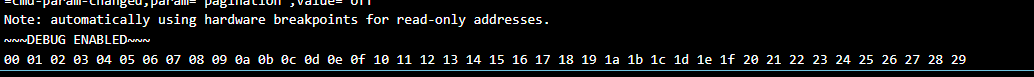
\includegraphics[width=0.5\linewidth]{RS485Debugg.png}
    \caption{This is my debug output I send a tx and output the rx in debug}
    \label{fig:enter-label}
\end{figure}
so I suppose that is it. I am ready to show I have that done at the meeting tomorrow. I was wanting to tinker more after relaxing with some video games. I decided to try setting up a breadboard with the usb power attach it to SERCOM4 and one of the RS485 clickks on a breadboard. I powered it from the click base board not the usb connected nano. I managed to get it to read the tx of the seconds on the other nano.
\begin{figure}
    \centering
    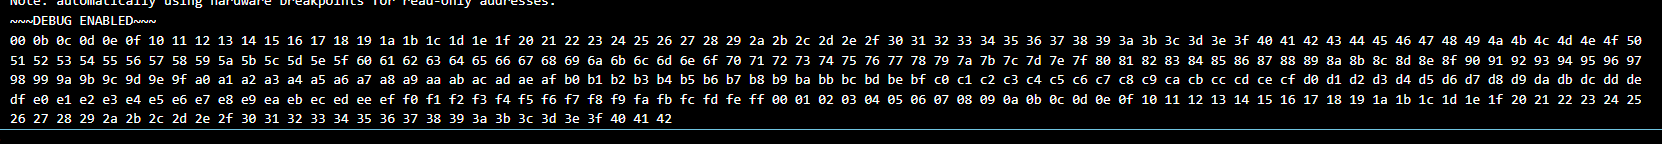
\includegraphics[width=0.5\linewidth]{RS485Debugg2.png}
    \caption{A long run of the debug print with two different nanos}
    \label{fig:enter-label}
\end{figure}
\begin{figure}
    \centering
    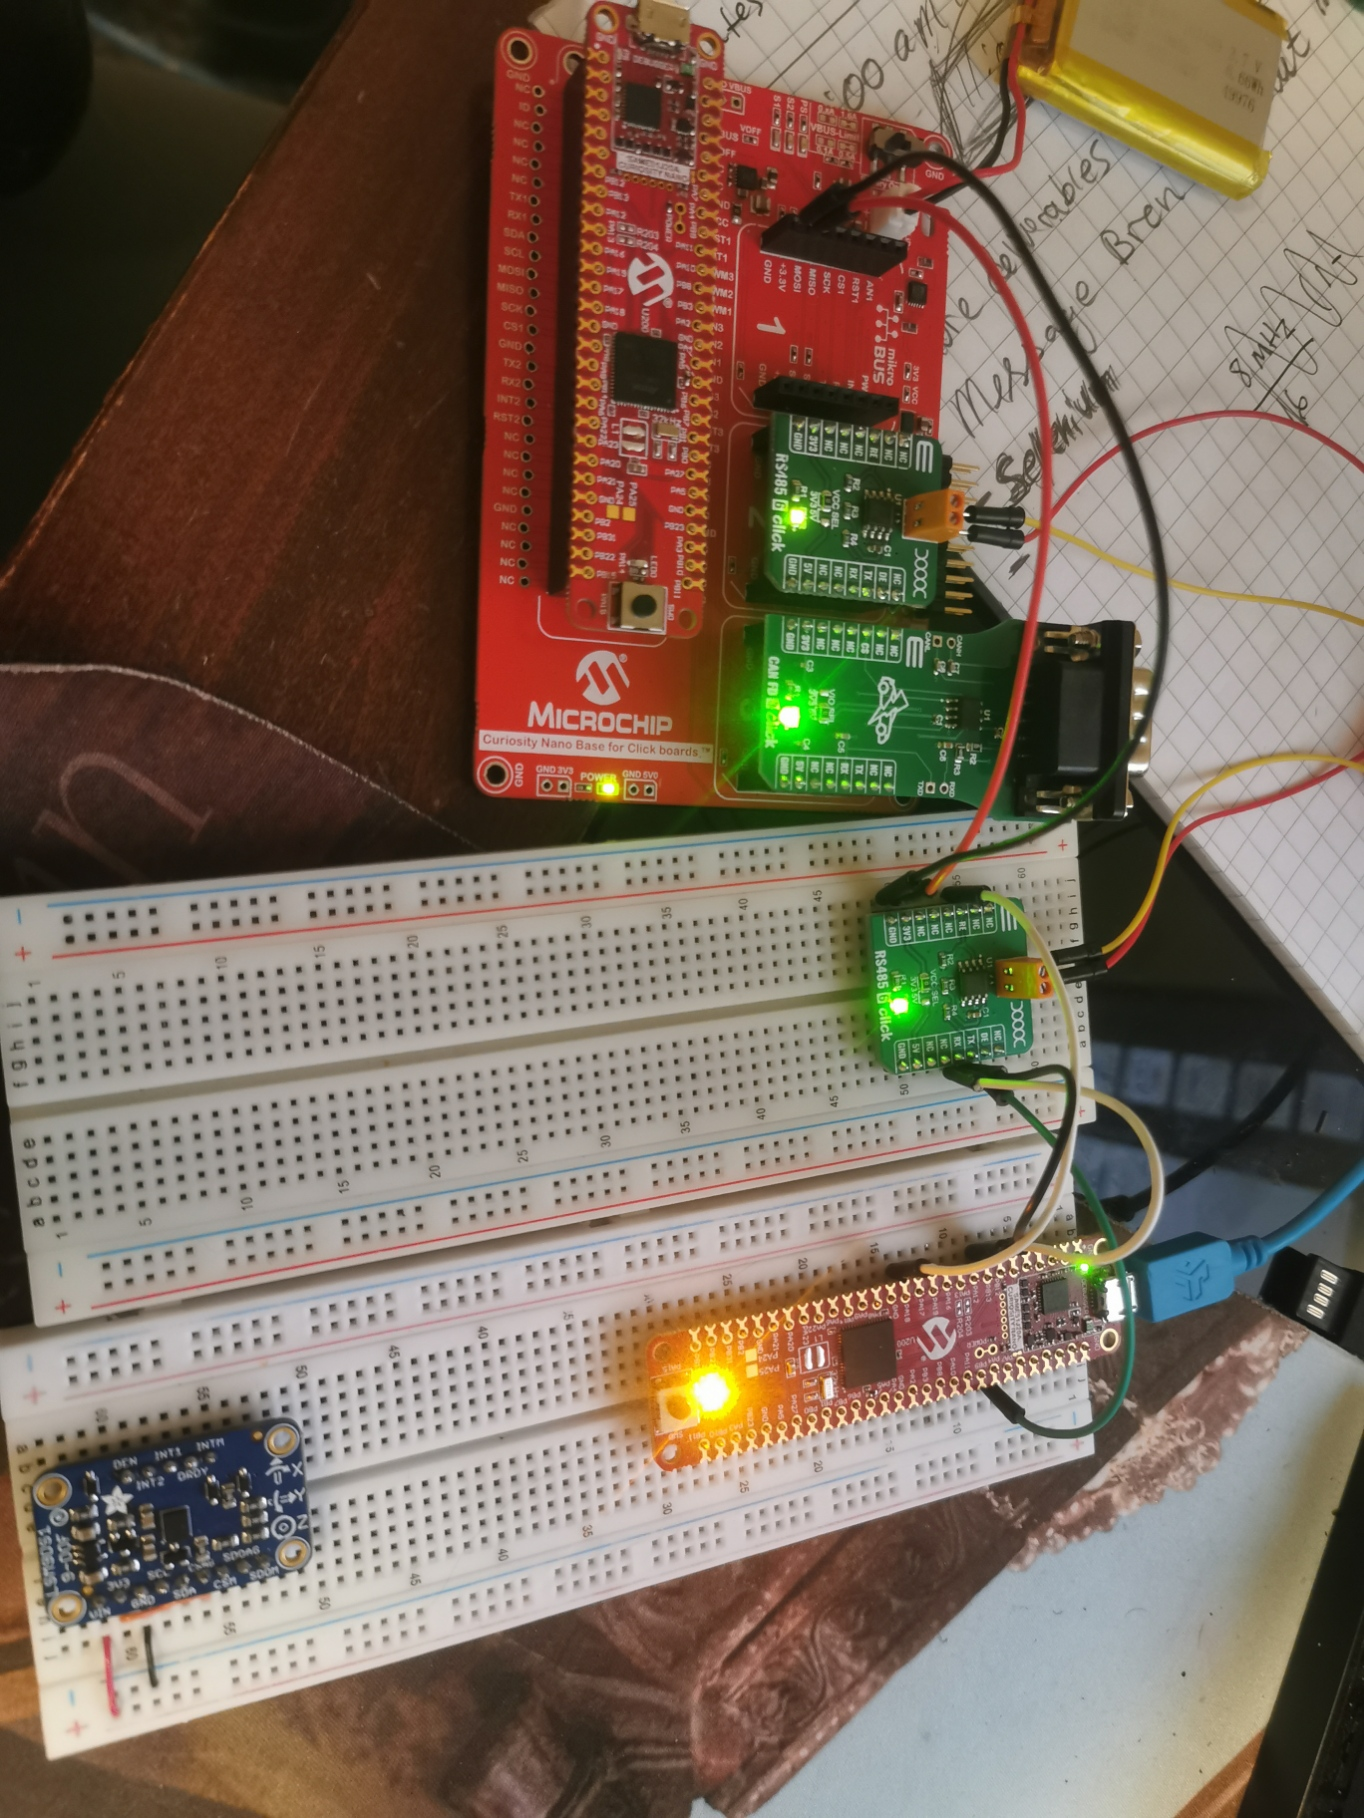
\includegraphics[width=0.5\linewidth]{setup-2-nano.jpg}
    \caption{2 nano setup}
    \label{fig:enter-label}
\end{figure}

\subsection{CAN Overview}
\paragraph{Controller Area Network (CAN)} is a standard for micro-controller and device communication. It uses messages, and was originally designed as a multiplexing method. The physical layer utilises twisted pairs (CAN+ and CAN-). Messages are framed with IDs which dictate priority. Logical 0 is Dominant and logical 1 is recessive. This means IDs that have larger values (1's in high bit places) are lower priority. Arbitration is done via first bit with a 1. All nodes see transmission.
\paragraph{Nodes} All nodes can send and receive, but not at the same time. The priority is determined by the frame ID. Messages are transmitted using non-return-to-zero (NRZ) format \\ All nodes require the following: 
\begin{itemize}
    \item Some controller :CPU/Microprocessor/host processor/micro controller
        \begin{itemize}
            \item Decides what messages mean and what to transmit
            \item Handles talking to other devices
        \end{itemize}
    \item CAN Controller
        \begin{itemize}
            \item Receiving: Stores bits until entire message is received, then can trigger interrupt for retrieval
            \item Transmitting: If the host, can send messages via CAN controller in a serial manner.
        \end{itemize}
    \item Transceiver (ISO 11898-2/3) Medium Access Unit (MAU)
        \begin{itemize}
            \item Receiving: converts at the CAN bus level for CAN controller use, protective layer for CAN controller. 
            \item Transmitting: converts bit stream from CAN controller to the CAN bus
        \end{itemize}
\end{itemize}



\subsection{CAN: IDs and arbitration}
\paragraph{ID Arbitration} When nodes transmit they see all messages including their own. If they transmit a 1 and see 0 they quit and lose arbitration. This is because 0 is dominant and they then know they do not have priority. Because of this, whenever there is a collision the lower ID will win. When a collision does happen.
The recessive message waits for the dominant message + 6-bit clocks then
attempts again
This means the first frame to transmit a 1 is the loser, thus highest
priority id frame is all 0s followed by 00\ldots.001
\paragraph{IDs as priorities}
Using ID for the type of data, or the sending node ignores the fact ID is
also used as message priority. This leads to poor real-time performance.
CAN bus is limited to around 30\% to ensure deadlines if you don't build
around the priority. Otherwise, you can achieve 70 to 80\% CAN bus usage and
have reliable deadlines.

\subsection{CAN: Bit timing}
\paragraph{Nominal Bit Time:} Time it takes to send bit components:\\

\paragraph{Synchronization} Synchronization is important to the CAN protocol. It prevents errors and allows for arbitration's to occur. Recolonization occurs every single recessive to dominant transmission during the frame. In order to sync the nominal bit time is segmented into quanta and then certain aspects can be altered to allow for synchronization. 
The nominal bit time is broken down in the following way. Each are assigned a number of quanta. For example a system where we break our nominal bit time into 10 quanta.


Sync (1 quanta)

Propagation (3 quanta)

Phase segment 1 (3 quanta)
 
Phase segment 2 (3 quanta)


Synchronization occurs as follows. 

\begin{enumerate}
\def\labelenumi{\arabic{enumi}.}
\item
  \textbf{Bus Idle} -\textgreater{} wait for first recessive to dominant
  transition
\item
 \textbf{ Hard synchronization}
\item
  \textbf{Resync} occurs on every recessive to dominant transition during the
  frame (message?)

  \begin{enumerate}
  \def\labelenumii{\alph{enumii}.}
  \item
    CAN controller expects this at multiple of nominal bit time.
  \item
    Else It adjust nominal bit time accordingly.
  \end{enumerate}
\end{enumerate}

~

\paragraph{Resync and Adjustment process:}

\begin{itemize}
\item
  Produce a number of quanta to divide the bits\textquotesingle{}
  segments into time slices.

  \begin{itemize}
  \item
    The number of quanta can vary based on the controller
  \item
    The quantity of quanta a segment is assigned can vary depending on
    system needs
  \end{itemize}
\item
  On out-of-sync (before or after) transition controller calculates the time
  difference, to compensate:

  \begin{itemize}
  \item
    If we need to lengthen we do so to phase 1
  \item
    If we need to reduce time we do so in phase 2.
  \end{itemize}
\item
  As a result of either a or b, we have adjusted the timing of the
  receiver to the transmitting node and synchronized them.
\item
  We continuously do so at every recessive to dominant transition to
  keep synchronization

  \begin{itemize}
  \item
    This reduces errors induced by noise (random error)
  \item
    Allows for resync to nodes that lost arbitration back to the one
    that won previously.
  \item
  \end{itemize}
\end{itemize}

\subsection{CAN Protocol Layers:}
\begin{itemize}
    \item Application layer
    \item Object layer
    \item Transfer layer
    \item Physical layer
\end{itemize}


We are building the transfer layer?

~

\subsubsection{CAN Transfer layer:}

\begin{itemize}
\item
  Most of the CAN standard applies to this layer, it is what receives
  messages from the physical layer and into the object layer for use in
  the application.
\item
  Transfer layer is responsible for:

  \begin{itemize}
  \item
    Synchronization
  \item
    Bit timing
  \item
    Message framing
  \item
    Arbitration
  \item
    Acknowledgement
  \item
    Error Detection
  \item
    Signalling
  \item
    Confinement
  \end{itemize}
\item
  To accomplish the previous responsibilities, it performs the following
  tasks:

  \begin{itemize}
  \item
    Fault confinement
  \item
    Error detection
  \item
    Message Validation
  \item
    Arbitration
  \item
    Message framing
  \item
    Transfer rate and timing
  \item
    Information routing
  \end{itemize}
\end{itemize}

~

Physical layer

\begin{itemize}
\item
  Pinout:

  \begin{itemize}
  \item
    Pin 2: CAN- (Low)
  \item
    Pin 3: GND
  \item
    Pin 7: CAN+ (High)
  \item
    Pin 9: CAN V+ (power)
  \end{itemize}
\end{itemize}

\begin{quote}
~
\end{quote}

\subsection{CAN Frames:}

\begin{itemize}
\item
  Two types of frame format

  \begin{enumerate}
  \def\labelenumi{\arabic{enumi}.}
  \item
    Base frame format

    \begin{enumerate}
    \def\labelenumii{\roman{enumii}.}
    \item
      11- bits for identifier
    \item
      IDE bit dominant
    \end{enumerate}
  \item
    Extended frame format

    \begin{enumerate}
    \def\labelenumii{\roman{enumii}.}
    \item
      11- bit identifier + 18-bit extension = 29-bit identifier
    \item
      IDE bit recessive
    \end{enumerate}
  \end{enumerate}
\item
  There are four types of frames.
\item
  Regardless of type all begin with a start of frame (SOF) bit to signal
  start of frame transmission.
\item
  Frame types:

  \begin{enumerate}
  \def\labelenumi{\arabic{enumi}.}
  \item
    Data Frame: a frame containing node data for transmission
    .

  \item
    Remote frame: requests transmission of an identifier
  \item
    Error frame: frame type for any node detecting an error.
  \item
    Overload frame: a buffer/delay for data or remote frame.
  \end{enumerate}
\end{itemize}
\begin{figure}
    \centering
    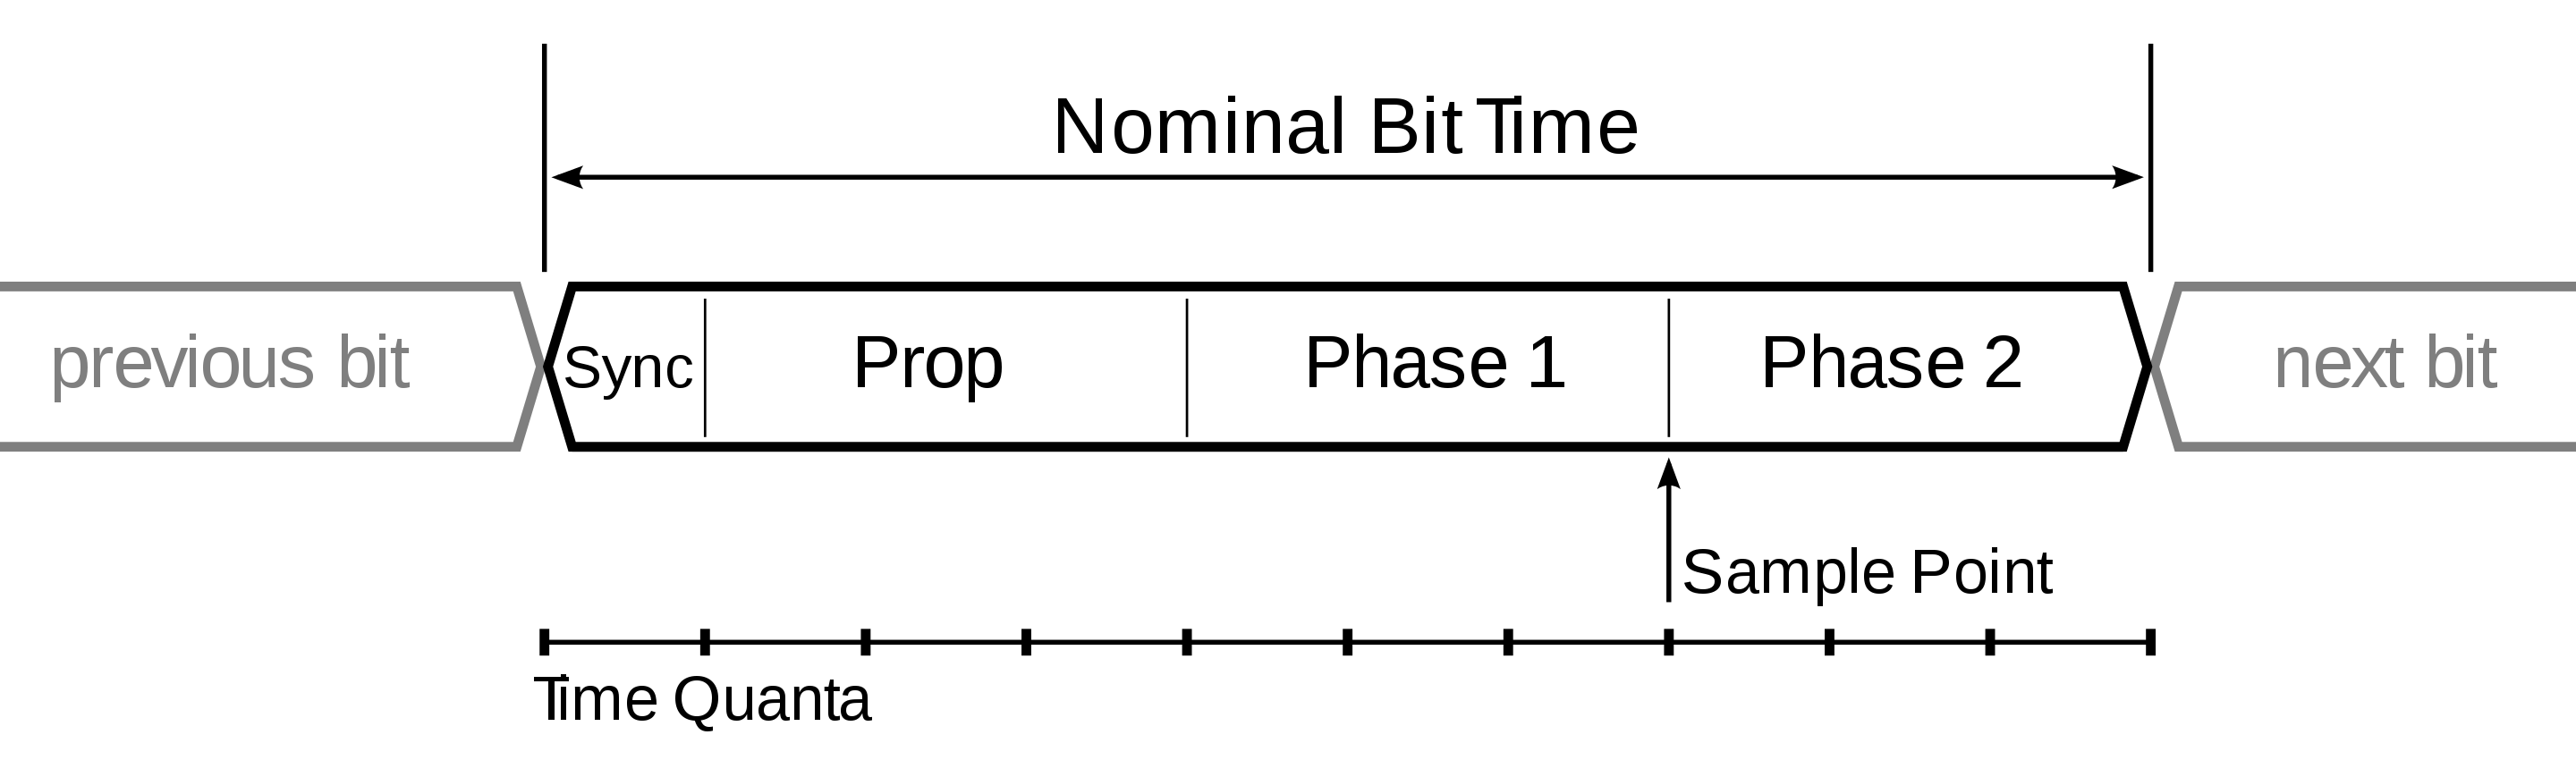
\includegraphics[width=1\linewidth]{2880px-CAN_Bit_Timing2.svg.png}
    \caption{CAN Bit Timing: Wikipedia}
    \label{fig:enter-label}
\end{figure}
\begin{figure}
      \centering
      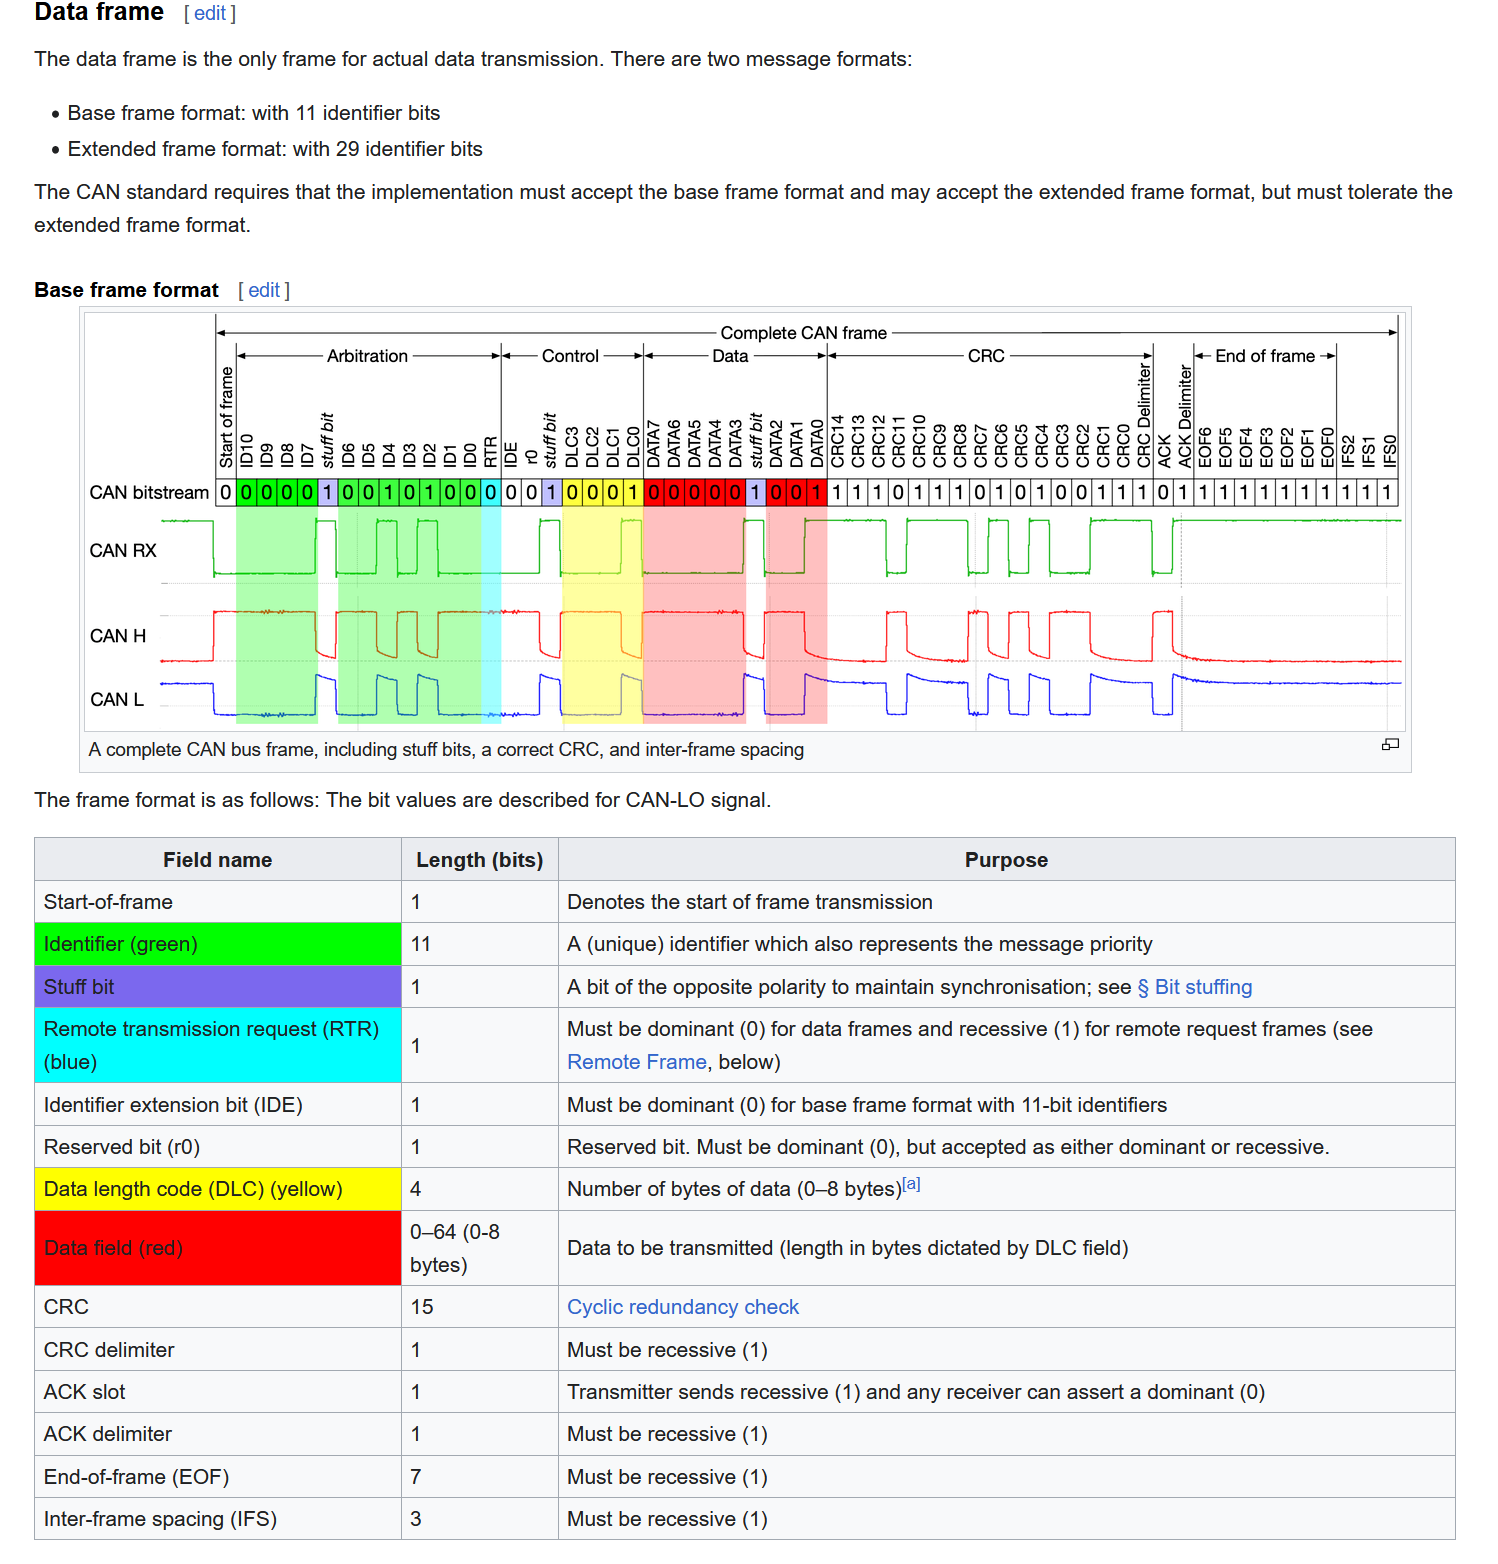
\includegraphics[width=1\linewidth]{Dataframe.png}
      \caption{Data frame: Wikipedia}
      \label{fig:enter-label}
  \end{figure}




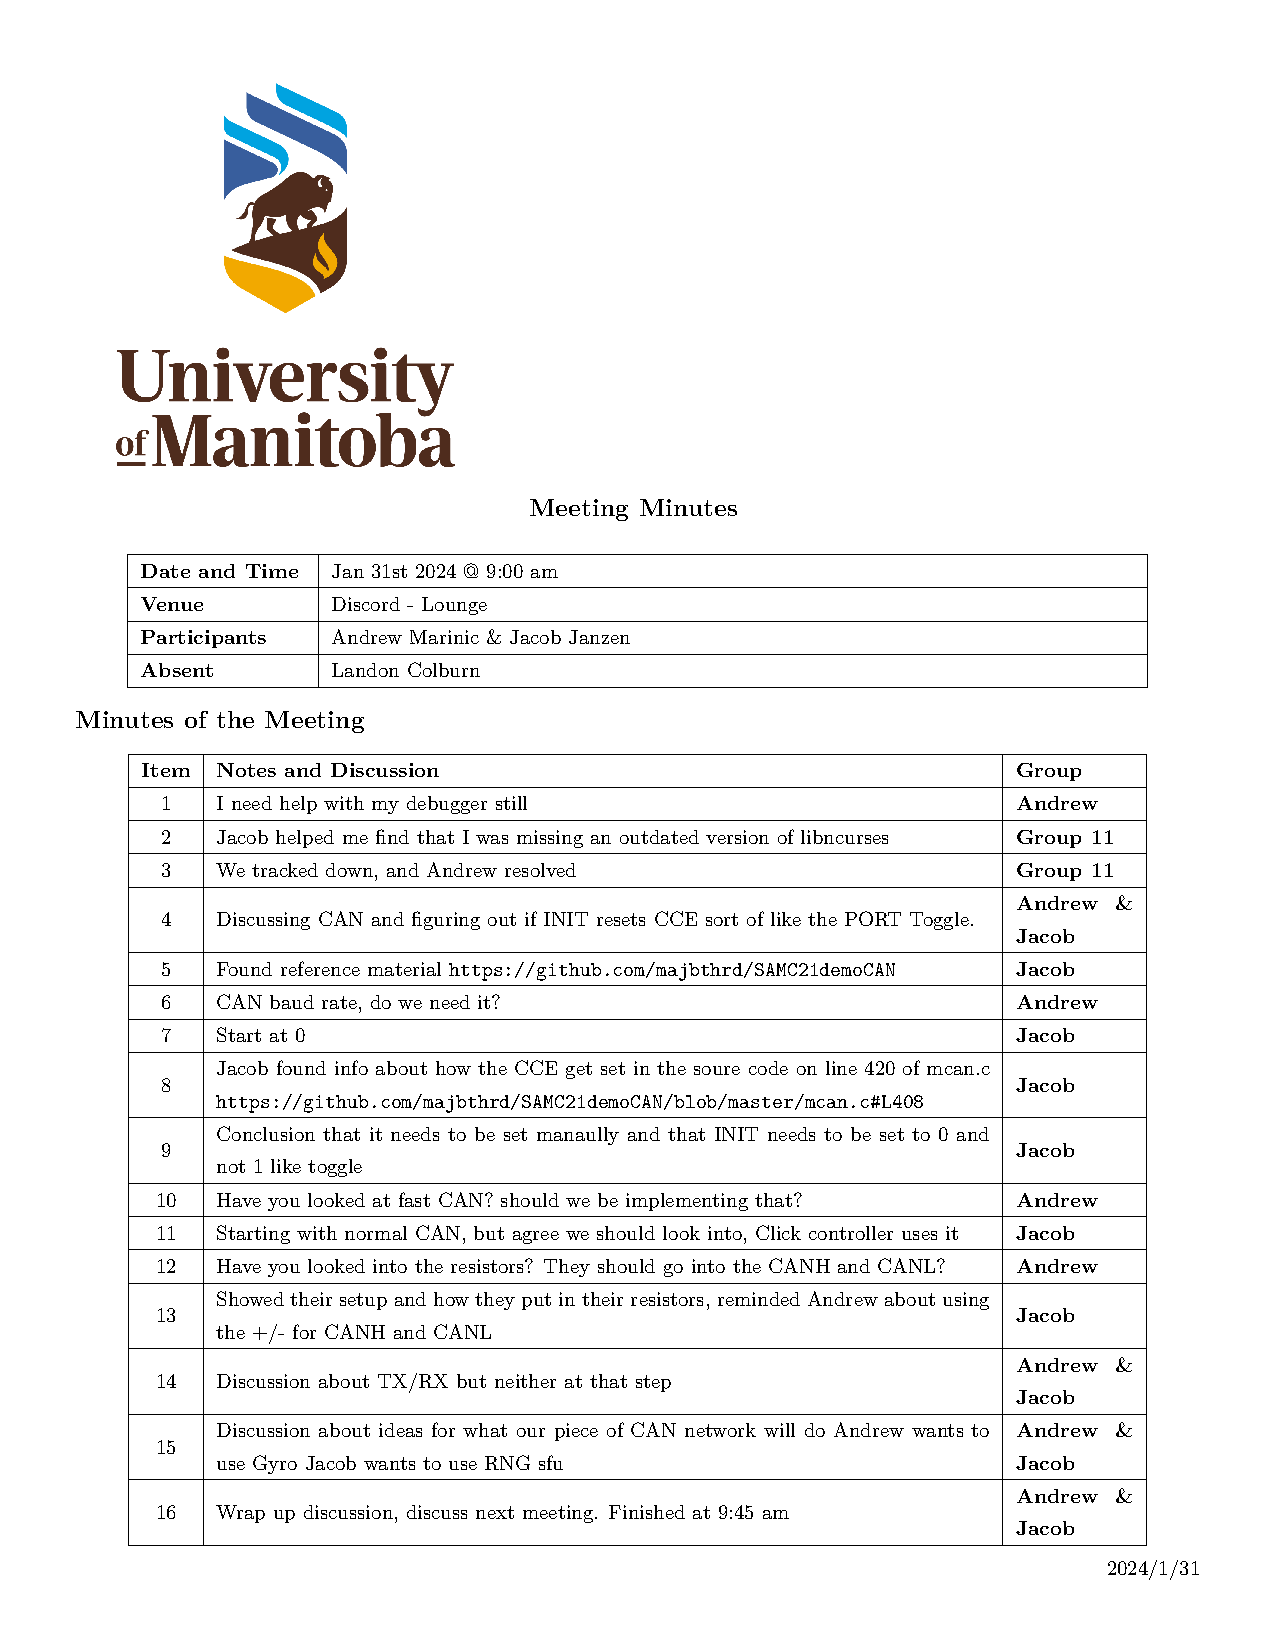
\includepdf[]{MeetingMinutes/Jan31/Jan31.pdf}
\subsection{RS485-6-Click}
\paragraph{General description} Uses the THVD1429DT (transceiver from TI) half-duplex RS485 via UART, rate of up to 20 Mbps. Voltage 3.3V to 5V. I can thus be useful for multi-point implementations, with tolerance to noise and  high physical distance integrity, achieved with a transient voltage suppressor. Each end should be terminated with a resistor that matches cable impedance. This parallel termination allows for the distance integrity. The total amount of BUS Nodes supported is 256. THe device has electrostatic discharge protection. Additionally it supports Electrical Fast Transient (EFT) protection which allows protection from high frequency bursts caused bu devices such as relays, switch contractors, or Heavy Duty Motors; additional surge transient protection from system power downs or short. Onboard voltage select interface available for 3.3v and 3v micro controllers. Interface to the device is available via UART. mikroBUS compatibility. 

\begin{figure}
    \centering
    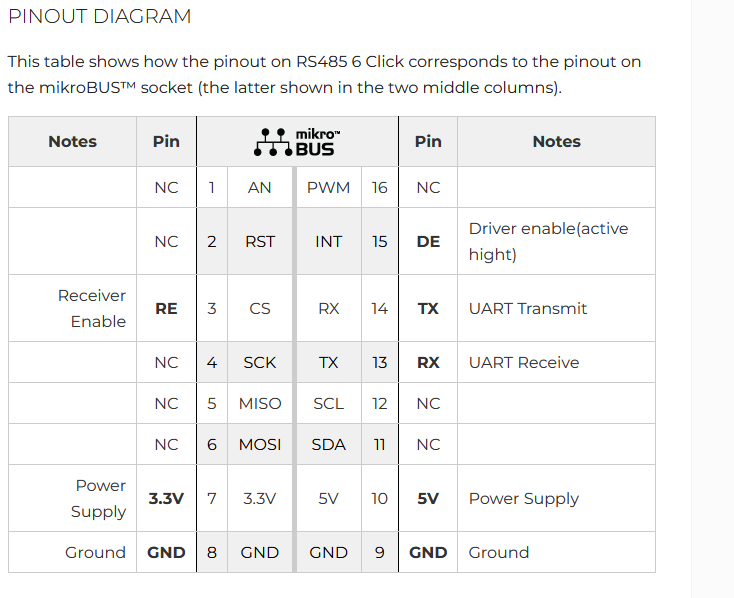
\includegraphics[width=0.5\linewidth]{rs485-pod.png}
    \caption{RS485-6 Pinout Diagram Source: https://www.mikroe.com/rs485-6-click}
    \label{fig:enter-label}
\end{figure}
\begin{figure}
    \centering
    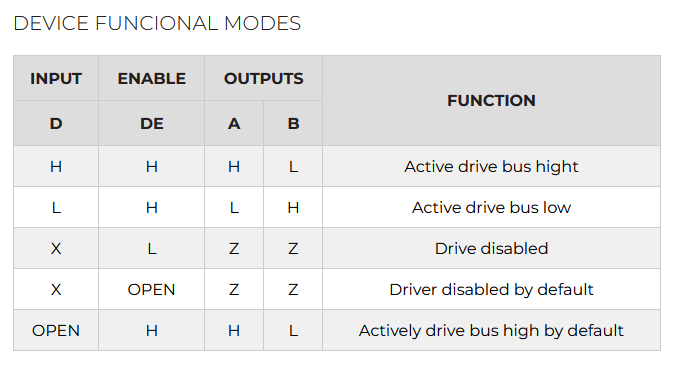
\includegraphics[width=0.5\linewidth]{rs485-dfm.png}
    \caption{RS485-6 Device Funcional Modes: https://www.mikroe.com/rs485-6-click}
    \label{fig:enter-label}
\end{figure}
\subsubsection{RS485-6-Click references}
\url{https://www.mikroe.com/rs485-6-click}
\url{https://libstock.mikroe.com/projects/view/3207/rs485-6-click}
\end{document}